\section{Results}

\subsection{Network Benchmarks}

\begin{figure*}
	\centering
	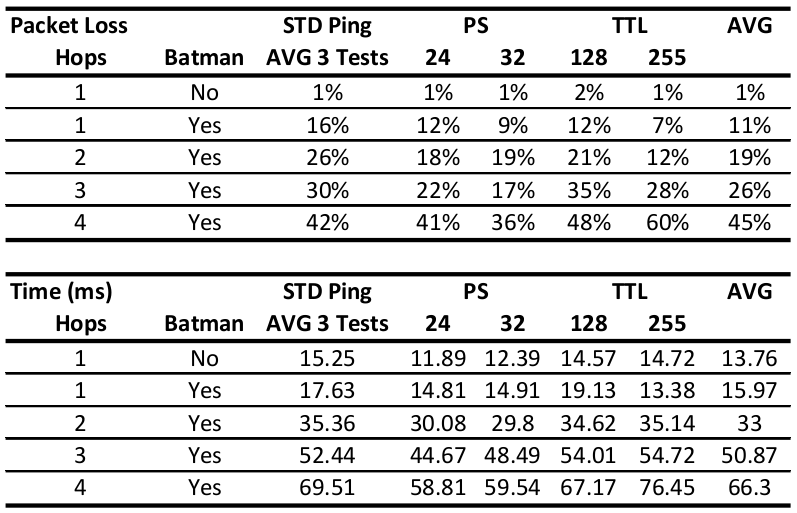
\includegraphics[scale=0.4]{902sheet}
	\caption{The data received from operating at 902/915 MHz.}
	\label{fig:902}
\end{figure*}

\begin{figure*}
	\centering
	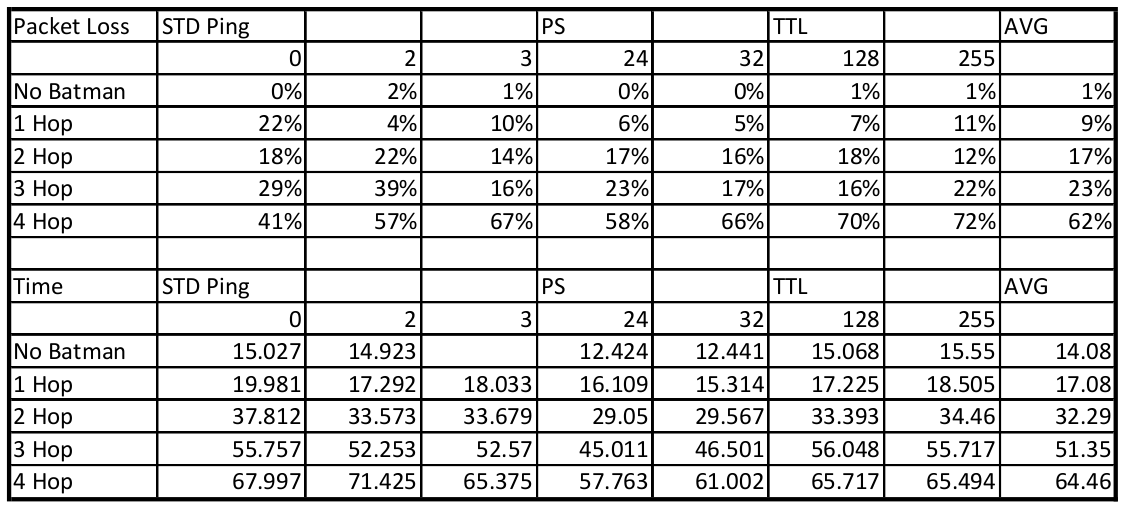
\includegraphics[scale=0.4]{2400}
	\caption{The data received from operating at 2.4/2.5 GHz.}
	\label{fig:2400}
\end{figure*}

\begin{figure}
	\centering
	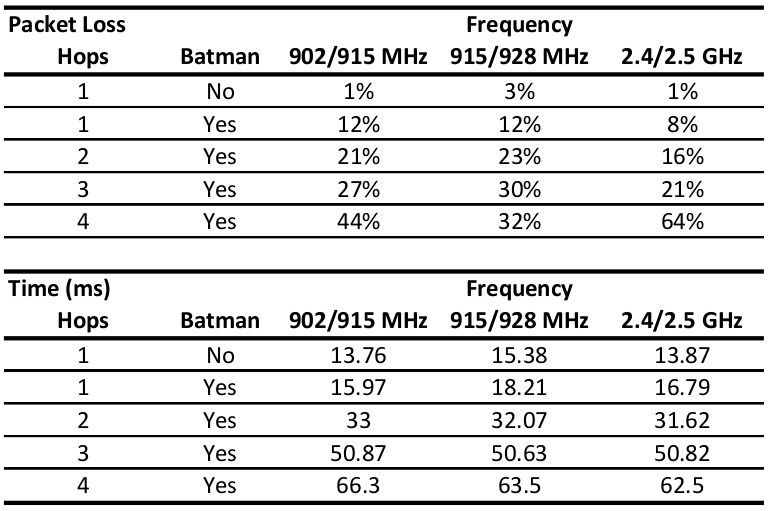
\includegraphics[scale=0.4]{alldata}
	\caption{The Averages from all three tests.}
	\label{fig:alldata}
\end{figure}

The results of the Network Benchmark tests are summarized in Figure \ref{fig:alldata}. In all cases, a single point to point communication, without the Batman-adv protocol running, resulted in a much lower packet loss. However, it is intersting to see that in the two sets of lower frequency raitings, the packet loss remained below 50\%. Also, the increase in time as hops were added has a roughly linear change. This is good as it means the overhead of adding more hops is not unmanageable. A full listing of tests run for the 902/915 MHz, and 2.4/2.5 GHz cases are provided in Figure \ref{fig:902} and Figure \ref{fig:2400} respectively. These tables show that running at the higher frequencies causes the SDRs to drop a lot more packets, especially when moving through the full four hops.  


\subsection{Route Changes}

\begin{figure*}
	\centering
	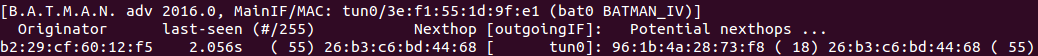
\includegraphics[scale=0.5]{2PotentialHops}
	\caption{The initial condition, where there are two possible routes the packet can take.}
	\label{fig:2Hops}
\end{figure*}

\begin{figure*}
	\centering
	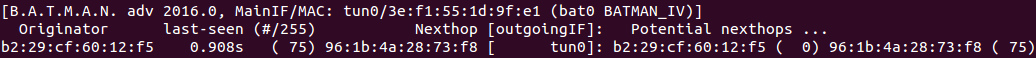
\includegraphics[scale=0.5]{hopchange}
	\caption{After the gain is reduced, the packets are now routing through a different node.}
	\label{fig:NewHop}
\end{figure*}

The route changing feature of Batman-adv worked very well with out test setup. As we decreased the gain of the intermediate node, the link quality reported by batctl also decreased. Eventually, Batman-adv switched and began using the other node. The initial setup can be seen in Figure \ref{fig:2Hops}. After the change, the routing table appeared as it does in Figure \ref{fig:NewHop}. This feature seems to work well even in the SDR system, and can likely be without much change.  

\subsection{Frequency Changes}

Using A.F.R.E.D. for frequency hopping showed mixed results. We were able to get the Nodes to change frequency in unison, but not reliably. A.F.R.E.D. itself is designed for a traditional Wi-Fi environment, and therefore does not have an expectation that the other nodes will become completely unreachable. We were finding that often times the nodes would switch well before A.F.R.E.D. had propagated the datatable to the other nodes. This would leave one node with an out of date table, meaning it would not make the frequency change. In the current iteration of the project, there was no way for these orphaned nodes to find the rest of the network again. Figure \ref{fig:freqshift} shows a situation in which four out of five nodes were able to make the jump, with one node remaining at the original frequency.

\begin{figure}
	\centering
	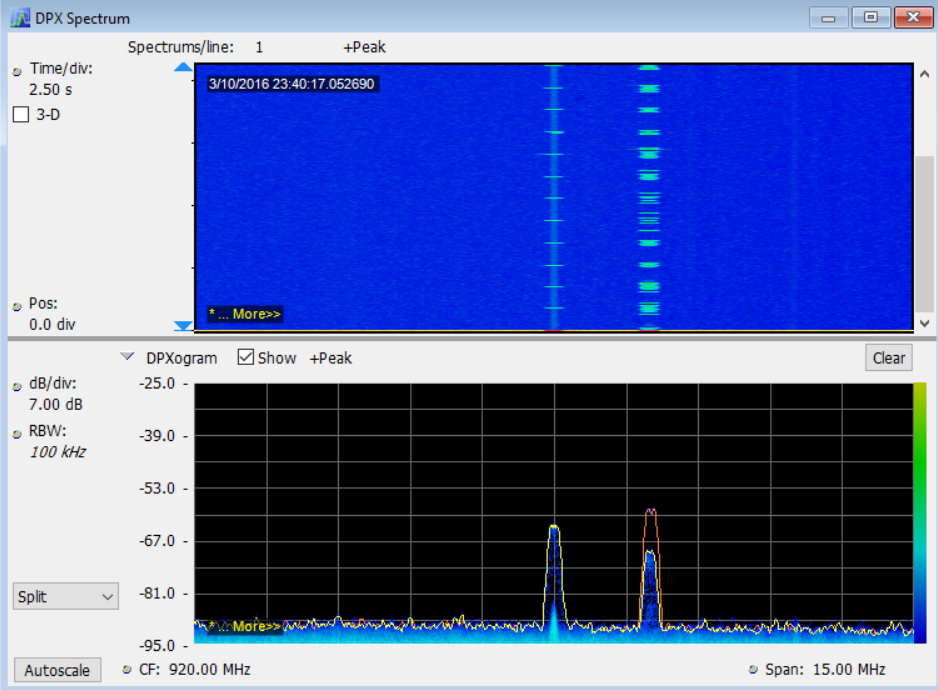
\includegraphics[scale=0.4]{FrequencyShift922-920}
	\caption{The result of using ALFRED to shift frequencies. One Node is left behind as the others move to the new channel.}
	\label{fig:freqshift}
\end{figure}


